\chapter{Description des propriétés fonctionnelles}
La Description des propriétés fonctionnelles (DPF), représenté par la figure \ref{fig:dpf}, permet de visualiser les exigences du client ainsi que de les associer aux fonctionnalités du produit.
Les relations entre les exigences et les fonctionnalités sont représentées par des chiffres de 1 (faible) à 5 (élevé).



\begin{landscape}
  %\begin{center}
    \begin{figure}[h]
      \caption{Description des propriétés fonctionnelles}
      \label{fig:dpf}
      %\centering
      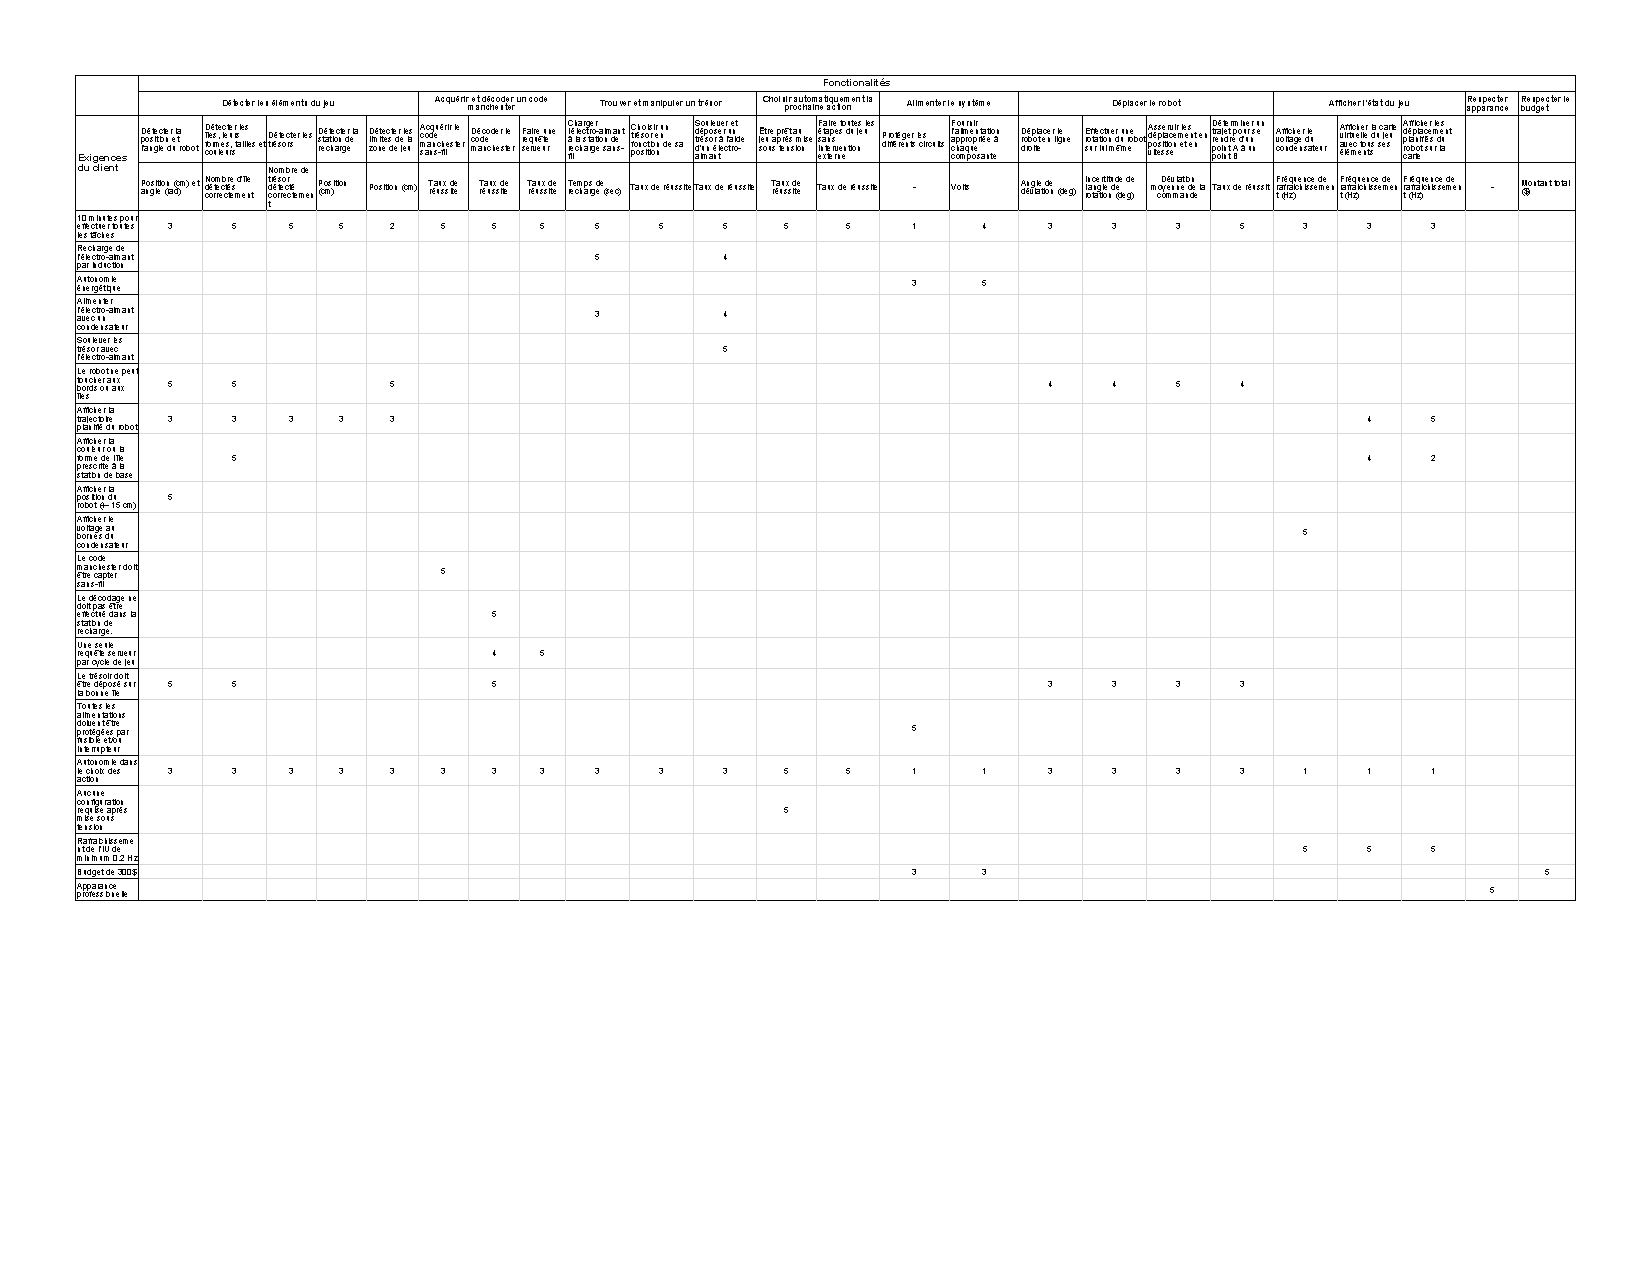
\includegraphics[scale=0.82]{resources/dpf.pdf}
    \end{figure}
  %\end{center}
\end{landscape}


\section{Détails des exigences}

\paragraph{10 minutes pour effectuer toutes les tâches:}
Le temps pour effectuer toutes les étapes d'un cycle de jeu est de 10 minutes. Le chronomètre part au moment où le signal de départ est donné au robot.
Plusieurs cycles de jeu peuvent être effectués durant les 10 minutes prescrits.

\paragraph{Recharge de l'électro-aimant par induction:}
Le condensateur qui va contenir la charge que l'électro-aimant va utiliser doit être rechargé par induction à la station de recharge.

\paragraph{Autonomie énergétique:}
Le robot doit être entièrement autonome du point de vue énergétique, donc alimenté seulement par la batterie.

\paragraph{Alimenter l'électro-aimant avec un condensateur:}
L'électro-aimant doit absolument être alimenté par un condensateur et non par un autre type d'alimentation.

\paragraph{Soulever les trésor avec l'électro-aimant:}
Le trésor doit être soulevé à l'aide d'un électro-aimant alimenté par un condensateur. La charge doit être suffisante afin de transporter le trésor jusqu'à l'île prescrite.

\paragraph{Le robot ne peut toucher aux bords ou aux îles:}
Dans tous ses déplacements, le robot ne peut toucher aux murs de la zone de jeu. Une seule offense est tolérée.

\paragraph{Afficher la trajectoire planifié du robot:}
Tous les déplacements du robot doivent être annoncés à l'avance.

\paragraph{Afficher la couleur ou la forme de l'île prescrite:} Une fois la requête serveur faite, le système doit afficher sur la station de base la couleur et la forme de l'île identifiée.

\paragraph{Afficher la position du robot:}
La position estimée du robot doit être affichée sur l'interface utilisateur. Cette position a une incertitude de 15 cm par rapport à la position réelle.

\paragraph{Afficher le voltage au bornes du condensateur:}
Le voltage du condensateur servant à alimenter l'électro-aimant doit être affiché sur l'interface utilisateur en tout temps.

\paragraph{Le code Manchester doit être capter sans-fil:}
La méthode d'acquisition du code Manchester doit être sans-fil, le spectre utilisé n'est pas important.

\paragraph{Le décodage ne doit pas être effectué dans la station de recharge:}
Il faut attendre que le condensateur soit plein avant de décoder le code Manchester.

\paragraph{Une seule requête serveur par cycle de jeu:}
Après l'aquisition du code Manchester, une seule requête serveur peut être faite par cycle de jeu.

\paragraph{Le trésor doit être déposé sur la bonne île:}
Le trésor doit être déposé sur l'île identifiée à l'aide du code Manchester et de la requête serveur.

\paragraph{Toutes les alimentations doivent être protégées par fusible et/ou interrupteur:}
Afin de protéger tout l'équipement du robot, toutes les alimentation se doivent d'être protégées au minimum par un fusible ou un interrupteur.

\paragraph{Autonomie dans le choix des actions:}
Durant tout le cycle de jeu, le robot doit être entièrement autonome dans ses déplacements et actions. Des touchettes sont autorisées avec pénalités.

\paragraph{Aucune configuration requise après mise sous tension:}
Après le démarrage, le robot doit commencer le jeu de manière autonome.

\paragraph{Rafraichissement minimal de l'interface utilisateur de 0.2 Hz:}
L'interface utilisateur affichant par exemple la position du robot, les trajets planifiés ainsi que le voltage du condensateur doit être rafraichit au minimum toutes les 5 secondes.

\paragraph{Budget de 300\$ :}
En dehors du matériel fourni, l'ensemble du matériel acheté servant au robot doit coûter au maximum 300\$.

\paragraph{Apparence professionnelle:}
L'ensemble des circuits doivent être montés sur circuits imprimés. Les breadboards ne sont pas permis.

\section{Détail des fonctionnalités}

\subsection{Détecter les éléments du jeu}

\paragraph{Détecter la position et l'angle du robot:}
Le robot est en mesure de se situer dans son environnement à l'aide des différents capteurs à sa disposition.

\paragraph{Détecter les îles, leurs formes, tailles et couleurs:}
Le robot détecte les îles placées de façon aléatoire. Il identifie leur dimension, leur couleur et leur forme.

\paragraph{Détecter les trésors:}
Le robot est en mesure de détecter les trésors dans l'environnement.

\paragraph{Détecter la station de recharge:}
Le robot peut identifier la station de recharge en début de cycle de jeu.

\paragraph{Détecter les limites de la zone de jeu:}
Le robot détecte lors de ses déplacement les limites de la zone de jeu afin de ne jamais entrer en contact avec elles.

\subsection{Acquérir et décoder un code Manchester}

\paragraph{Acquérir le code Manchester sans-fil:}
Le robot peut acquérir un code Manchester à l'aide d'un protocole HF.

\paragraph{Décoder le code Manchester:}
Le robot est en mesure de décoder le code Manchester afin d'obtenir le caractère ASCII correspondant.

\paragraph{Faire une requête serveur:}
Le robot peut effectuer une requête GET ayant comme paramètre le code reçu par le signal HF.

\subsection{Trouver et manipuler un trésor}

\paragraph{Charger l'électro-aimant à la station de recharge sans-fil:}
Le robot a un dispositif permettant de charger un condensateur par induction afin d'offrir de la puissance à l'électro-aimant.

\paragraph{Choisir un trésor en fonction de sa position:}
Avec ses capteurs, le robot est en mesure de choisir un des trésor sur la zone de jeu en fonction de sa position.

\paragraph{Soulever et déposer un trésor à l'aide d'un électro-aimant:}
Avec son électro-aimant, le robot est en mesure de soulever et de déposer un trésor.

\subsection{Choisir automatiquement la prochaine action:}

\paragraph{Être prêt au jeu après mise sous tension:}
Le robot doit être en mesure de jouer une fois que la mise sous tension est appliqué.

\paragraph{Faire toutes les étapes du jeu sans intervention externe:}
Le robot doit faire un cycle de jeu complet de manière autonome.

\subsection{Alimenter le système}

\paragraph{Protéger les différents circuits:}
Toutes les alimentation sont protégées avec des fusibles ou des interrupteurs.

\paragraph{Fournir l'alimentation appropriée à chaque composante:}
Chaque composante a des besoins différents en alimentation. Le robot possède donc une alimentation pour les moteur, l'ordinateur embarqué, la caméra embarquée, le micro-contrôleur, le pololu et l'électro-aimant.

\subsection{Déplacer le robot}

\paragraph{Déplacer le robot en ligne droite:}
Avec ses 4 roues, le robot est en mesure de se déplacer dans toutes les directions dans les axes X et Y.

\paragraph{Effectuer une rotation du robot sur lui même:}
Le robot peut tourner sur lui-même à gauche ou à droite.

\paragraph{Asservir les déplacements en position et en vitesse:}
Les 4 roues sont asservies en vitesse de façon à garder une vitesse constante correspondant à la commande.

\paragraph{Déterminer un trajet pour se rendre d'un point A à un point B:}
Pour un objectif avec une position donnée, le robot peut déterminer une série de mouvement à faire pour s'y rendre.

\subsection{Afficher l'état du jeu}

\paragraph{Afficher le voltage du condensateur:}
Le robot envoie à la station de base le voltage du condensateur qui l'affiche en temps réel.

\paragraph{Afficher la carte virtuelle du jeu avec tous ses éléments:}
La station de base affiche une carte correspondant à la zone de jeu et ses éléments, incluant la position estimée du robot.

\paragraph{Afficher les déplacements planifiés du robot sur la carte:}
Les déplacements calculé par le robot sont affichés sur la carte à la station de base.

\subsection{Respecter apparences}
Aucun breadboard n'est utilisé, tous les circuits sont fait sur PCB.

\subsection{Respecter le budget}
Toutes les composantes du robot respecte le budget total de 300\$.
